\documentclass[11pt]{article}
\usepackage{amssymb}
\usepackage{amsthm}
\usepackage{enumitem}
\usepackage{amsmath, physics}
\usepackage{bm}
\usepackage{adjustbox}
\usepackage{mathrsfs}
\usepackage{graphicx}
% \usepackage{siunitx}
\usepackage{physunits}
\usepackage[mathscr]{euscript}

\title{\textbf{Solved selected problems of Classical Electrodynamics - Hans Ohanian}}
\author{Franco Zacco}
\date{}

\addtolength{\topmargin}{-3cm}
\addtolength{\textheight}{3cm}

\newcommand{\Nat}{\mathbb{N}}
\newcommand{\Z}{\mathbb{Z}}
\newcommand{\Q}{\mathbb{Q}}
\newcommand{\R}{\mathbb{R}}
\newcommand{\diam}{\text{diam}}
\newcommand{\cl}{\text{cl}}
\newcommand{\bdry}{\text{bdry}}
\newcommand{\inter}{\text{int}}
\newcommand{\hatx}{\bm{\hat{x}}}
\newcommand{\haty}{\bm{\hat{y}}}
\newcommand{\hatz}{\bm{\hat{z}}}
\newcommand{\hatr}{\bm{\hat{r}}}
\newcommand{\hatn}{\bm{\hat{n}}}
\newcommand{\hatrho}{\bm{\hat{\rho}}}
\newcommand{\hatphi}{\bm{\hat{\phi}}}
\newcommand{\hattheta}{\bm{\hat{\theta}}}
\newcommand{\vecx}{\bm{x}}


\theoremstyle{definition}
\newtheorem*{solution*}{Solution}
\renewcommand*{\proofname}{\bf{Solution}}

\begin{document}
\maketitle
\thispagestyle{empty}

\section*{Chapter 2 - Electrostatics}

\subsection*{Exercises}

\begin{proof}{\textbf{Exercise 1.}}
    Below we show how to express the dyne per esu in centimeters, grams
    and seconds. 
    \begin{align*}
        \frac{\dyne}{\esu}
        = \frac{\gm\cm}{\s^2} \frac{1}{\cm\sqrt{\dyne}}
        = \frac{\gm\cm}{\s^2} \frac{\s}{\cm\sqrt{\gm\cm}}
        = \frac{1}{\s}\sqrt{\frac{\gm}{\cm}}
    \end{align*}
\end{proof}
\begin{proof}{\textbf{Exercise 2.}}
    Let us consider a sphere of radius $R$ with charge $Q$ uniformly
    distributed over its volume.
    
    Let us consider first the case where $r \leq R$ as shown below
    \begin{center}
        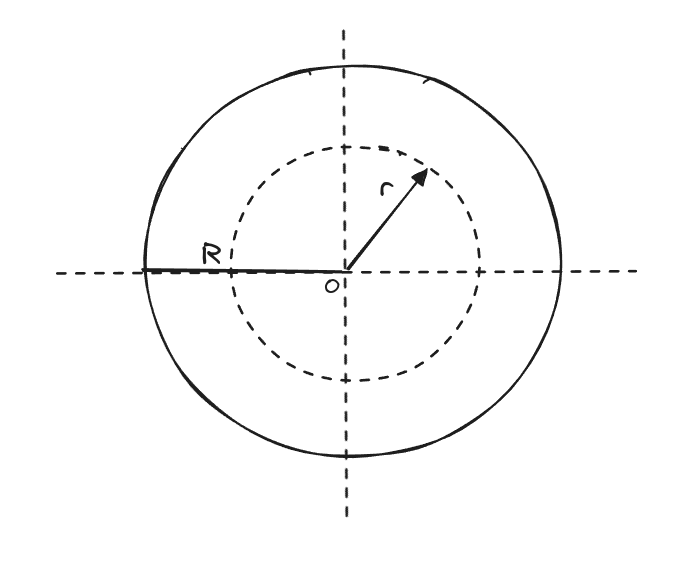
\includegraphics[scale=0.4]{ch2-ex2.png}
    \end{center}
    The charge per unit of volume is $3Q/4\pi R^3$ then the charge enclosed in
    the sphere of radius $r$ is
    $$\frac{3Q}{4\pi R^3} \frac{4\pi r^3}{3} = \frac{Qr^3}{R^3}$$
    On the other hand, we know that $\bm E(\bm{x}) = E\hatr$ where $E$ is the
    constant value of the electric field because of the symmetric distribution
    of charge.
    Hence Gauss' law in integral form is given by 
    \begin{align*}
        \int_{0}^{2\pi}\int_{0}^{\pi} E~r^2\sin\theta d\theta d\phi
        &= 4\pi\frac{Qr^3}{R^3}\\
        4\pi Er^2 &= 4\pi\frac{Qr^3}{R^3}\\
        \bm E &= \frac{Qr}{R^3}\hatr
    \end{align*}

    In the case where $r \geq R$ the enclosed charge is just $Q$ and applying
    again Gauss' Law we get that
    \begin{align*}
        \int_{0}^{2\pi}\int_{0}^{\pi} E~r^2\sin\theta d\theta d\phi
        &= 4\pi Q\\
        4\pi Er^2 &= 4\pi Q\\
        \bm E &= \frac{Q}{r^2}\hatr
    \end{align*}
\end{proof}
\cleardoublepage
\begin{proof}{\textbf{Exercise 3.}}
    We know that
    \begin{align*}
        \Phi(\vecx) = \frac{q'}{|\vecx - \vecx'|}
        = \frac{q'}{\sqrt{(x -x')^2 + (y -y')^2 + (z -z')^2}}
    \end{align*}
    So by applying the gradient to this equation we get that
    \begin{align*}
        \nabla\Phi(\vecx)
        &= \partialderivative{\Phi}{x}\hatx 
        + \partialderivative{\Phi}{y}\haty + \partialderivative{\Phi}{z}\hatz\\
        &= -\frac{q'(x- x')}{((x -x')^2 + (y -y')^2 + (z -z')^2)^{3/2}}\hatx\\
        &\quad -\frac{q'(y - y')}{((x -x')^2 + (y -y')^2 + (z -z')^2)^{3/2}}\haty\\
        &\quad -\frac{q'(z - z')}{((x -x')^2 + (y -y')^2 + (z -z')^2)^{3/2}}\hatz\\
        &= -\frac{q'((x -x')\hatx + (y -y')\haty + (z -z')\hatz)}
        {((x -x')^2 + (y -y')^2 + (z -z')^2)^{3/2}}\\
        &= -q'\frac{\vecx - \vecx'}{|\vecx - \vecx'|^3}
    \end{align*}
    Therefore
    \begin{align*}
        \bm{E}(\vecx) = -\nabla\Phi(\vecx)
        = q'\frac{\vecx - \vecx'}{|\vecx - \vecx'|^3}
    \end{align*}

    On the other hand, for a distributioon of charges with a charge density of
    $\rho(\vecx')$ we know that
    \begin{align*}
        \Phi(\vecx) = \int \frac{\rho(\vecx')}{|\vecx - \vecx'|} dV'
        = \int\frac{\rho(\vecx')}{\sqrt{(x -x')^2 + (y -y')^2 + (z -z')^2}} dV'
    \end{align*}
    Hence the gradient is
    \begin{align*}
        \nabla\Phi(\vecx)
        &= \partialderivative{\Phi}{x}\hatx 
        + \partialderivative{\Phi}{y}\haty + \partialderivative{\Phi}{z}\hatz\\
        &= \int\rho(\vecx')
        \partialderivative{}{x}
        \bigg(\frac{1}{\sqrt{(x -x')^2 + (y -y')^2 + (z -z')^2}}\bigg)dV'\hatx\\
        &\quad + \int\rho(\vecx')
        \partialderivative{}{y}
        \bigg(\frac{1}{\sqrt{(x -x')^2 + (y -y')^2 + (z -z')^2}}\bigg)dV'\haty\\
        &\quad + \int\rho(\vecx')
        \partialderivative{}{z}
        \bigg(\frac{1}{\sqrt{(x -x')^2 + (y -y')^2 + (z -z')^2}}\bigg)dV'\hatz\\
        &= -\int\rho(\vecx')
        \bigg(\frac{(x- x')}{((x -x')^2 + (y -y')^2 + (z -z')^2)^{3/2}}\hatx\\
        &\quad+ \frac{(y - y')}{((x -x')^2 + (y -y')^2 + (z -z')^2)^{3/2}}\haty\\
        &\quad+ \frac{(z - z')}{((x -x')^2 + (y -y')^2 + (z -z')^2)^{3/2}}\hatz
        \bigg)~dV'\\
        &= -\int\rho(\vecx')
        \bigg(\frac{(x- x')\hatx + (y - y')\haty + (z -z')\hatz}
        {((x -x')^2 + (y -y')^2 + (z -z')^2)^{3/2}}\bigg)~dV'\\
        &= -\int\rho(\vecx')
        \frac{\vecx - \vecx'}{|\vecx - \vecx'|^3}~dV'
    \end{align*}
    Therefore
    \begin{align*}
        \bm{E}(\vecx) = -\nabla\Phi(\vecx)
        = \int\rho(\vecx') \frac{\vecx - \vecx'}{|\vecx - \vecx'|^3}~dV'
    \end{align*}
\end{proof}
\cleardoublepage
\begin{proof}{\textbf{Exercise 4.}}
    We know the electric field of a sphere of radius $R$ an charge $Q$
    uniformly distributed over its volume is given by
    \begin{align*}
        \bm{E}(r) = Q\frac{\hatr}{r^2} \quad\quad r \geq R\\
        \bm{E}(r) = Q\frac{r\hatr}{R^3} \quad\quad r \leq R
    \end{align*}
    Then by using that
    \begin{align*}
        \Phi(\vecx) = - \int_{x_0}^x E(\vecx')\cdot d\vecx'
    \end{align*}
    We can compute the electrostatic potential $\Phi$ for $r \geq R$ as follows
    \begin{align*}
        \Phi(r) &= - \int_{\infty}^r Q\frac{\hatr}{r'^2}\cdot \hatr dr'\\
        &= - Q\bigg[-\frac{1}{r'}\bigg]_{\infty}^r\\
        &= - Q\bigg[-\frac{1}{r} + 0\bigg]\\
        &= \frac{Q}{r}
    \end{align*}
    And for $r \leq R$ we have that
    \begin{align*}
        \Phi(r) &= - \int_{\infty}^R Q\frac{\hatr}{r'^2}\cdot \hatr dr'
        - \int_{R}^r Q\frac{r'\hatr}{R^3}\cdot \hatr dr'\\
        &= - Q\bigg[-\frac{1}{r'}\bigg]_{\infty}^R
        - \frac{Q}{R^3}\bigg[\frac{r'^2}{2}\bigg]_{R}^r\\
        &= Q\bigg[\frac{1}{R}\bigg] 
        - \frac{Q}{R^3}\bigg[\frac{r^2}{2} - \frac{R^2}{2}\bigg]\\
        &= Q\bigg[\frac{1}{R} - \frac{r^2}{2R^3} + \frac{1}{2R}\bigg]\\
        &= Q\bigg[- \frac{r^2}{2R^3} + \frac{3}{2R}\bigg]
    \end{align*}
\end{proof}
\begin{proof}{\textbf{Exercise 5.}}
Below we show how to express a statvolt in centimeters, grams and seconds.
    \begin{align*}
        1~\text{statvolt} = \frac{1~\text{erg}}{1~\text{esu}}
        = \frac{1~\dyne \cm}{1~\cm\sqrt{1~\dyne}}
        % = \frac{1~\dyne}{\sqrt{1~\dyne}}
        = \frac{1~\text{g}\cm / \text{s}^2}{1~(\text{g}\cm)^{1/2} / \text{s}}
        = 1~\frac{(\text{g}\cm)^{1/2}}{\text{s}}
    \end{align*}
\end{proof}
\cleardoublepage
\begin{proof}{\textbf{Exercise 6.}}
    We know that 
    \begin{align*}
        \nabla \times \bm{E} = \varepsilon^{mrs} \partialderivative{}{x^r} E^s
    \end{align*}
    Hence
    \begin{align*}
        \bm{p} \times (\nabla \times \bm{E})
        &= \varepsilon^{klm} p^l (\varepsilon^{mrs} \partialderivative{}{x^r} E^s)\\
        &= \varepsilon^{klm} \varepsilon^{mrs} p^l(\partialderivative{}{x^r} E^s)\\
        &= (\delta^{kr}\delta^{ls} - \delta^{ks}\delta^{lr})(p^l\partialderivative{}{x^r} E^s)\\
        &= (p^l\partialderivative{}{x^k}E^l) - (p^l\partialderivative{}{x^l}E^k)\\
        &= \partialderivative{}{x^k}~(p^lE^l) - (p^l\partialderivative{}{x^l}E^k)\\
        &= \nabla(\bm{p}\cdot\bm{E}) - (\bm{p}\cdot\nabla)\bm{E}
    \end{align*}
    If $\curl \bm{E} = 0$ we get that
    \begin{align*}
        \nabla(\bm{p}\cdot\bm{E}) - (\bm{p}\cdot\nabla)\bm{E} &= 0\\
        \nabla(\bm{p}\cdot\bm{E}) &= (\bm{p}\cdot\nabla)\bm{E}
    \end{align*}
    Which implies that the equations (61) and (64) are equivalent.
\end{proof}
\cleardoublepage
\begin{proof}{\textbf{Exercise 7.}}
    Let $U = -pE\cos\theta$ then by differentiation we have that
    \begin{align*}
        \partialderivative{U}{\theta} = pE\sin\theta
    \end{align*}
    Hence this is a torque in the normal direction to $\bm{p}$ and $\bm{E}$ i.e.
    \begin{align*}
        \bm{\tau} = pE\sin\theta~\bm{n} = \bm{p} \times \bm{E}
    \end{align*}
\end{proof}

\end{document}